%
% File: chap02.tex
%
\let\textcircled=\pgftextcircled
\chapter{Results}
\label{chap:result}

\initial{I}n this section, the results are given. And they're shit. This presents what results are shown, etc. Not much to say actually, besides showing the plot. THis is a simple lab. We discuss about the uncertainties too.

\section{Results}

\begin{figure}[t!]
	\centering
	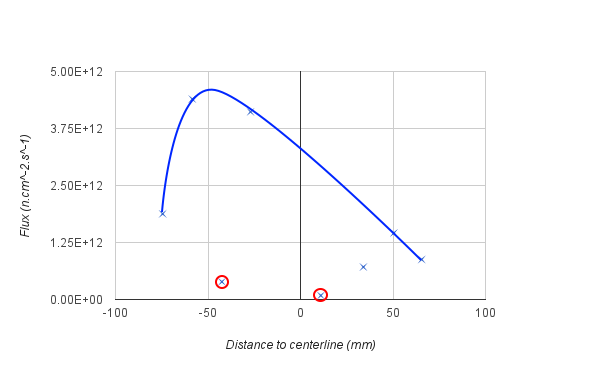
\includegraphics[height=0.4\textheight]{fig02/flux1.png}
	\mycaption[Thermal neutron flux seen in the samples]{Thermal neutron flux seen in the samples.}
	\label{fig:flux1}
\end{figure}

\begin{figure}[t!]
	\centering
	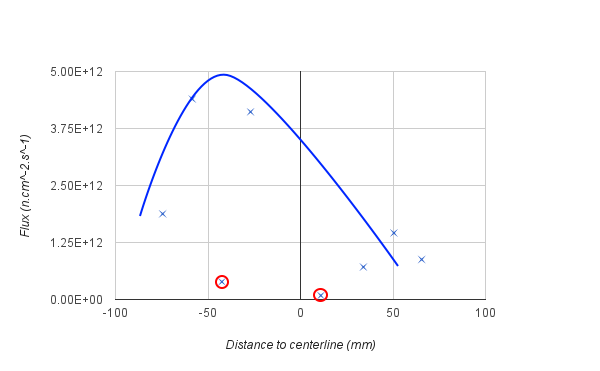
\includegraphics[height=0.4\textheight]{fig02/flux2.png}
	\mycaption[Thermal neutron flux seen in the samples]{Thermal neutron flux seen in the samples.}
	\label{fig:flux2}
\end{figure}

\section{Uncertainties}


